\def\year{2015}
%File: formatting-instruction.tex
\documentclass[letterpaper]{article}
\usepackage{aaai}
\usepackage{times}
\usepackage{helvet}
\usepackage{courier}
\usepackage{url}
\usepackage{array}
\usepackage{graphicx}
\newcolumntype{L}[1]{>{\raggedright\let\newline\\\arraybackslash\hspace{0pt}}m{#1}}
\newcolumntype{C}[1]{>{\centering\let\newline\\\arraybackslash\hspace{0pt}}m{#1}}
\newcolumntype{R}[1]{>{\raggedleft\let\newline\\\arraybackslash\hspace{0pt}}m{#1}}
\newcommand{\specialcell}[2][l]{%
  \begin{tabular}[#1]{@{}l@{}}#2\end{tabular}}
\frenchspacing
\setlength{\pdfpagewidth}{8.5in}
\setlength{\pdfpageheight}{11in}
\pdfinfo{
/Title Pre-orders or Philanthropy: An Analysis of Altruism on Kickstarter
/Author Jack Hessel
/Keywords X,Y,Z}
\setcounter{secnumdepth}{0}  
 \begin{document}
% The file aaai.sty is the style file for AAAI Press 
% proceedings, working notes, and technical reports.
%
\title{Pre-orders or Philanthropy: An Analysis of Altruism on Kickstarter}
\author{Jack Hessel \and Lillian Lee\\Cornell University}
\maketitle
\begin{abstract}
\begin{quote}
Abstract
\end{quote}
\end{abstract}

\section{Introduction}

In recent years, crowdfunding websites have emerged as a popular method of fundraising for individuals looking to promote their ventures to online communities. The most popular of these sites, Kickstarter, provides a venue for entrepreneurs to connect with individuals who might be interested in financially supporting their project ideas, which range from artistic endevours to technology startups. To date, over \$1.4B has been invested in Kickstarter projects from more than 7.4M unique backers resulting in over 73K successfully funded projects. \footnote{ \url{www.kickstarter.com/help/stats}} Each project is associated with a set of creator-defined rewards that donors can choose from. Often, these rewards constitute pre-orders of a product that the project aims to bring to market.

(PARAGRAPH ABOUT ACADEMIC INTEREST WITH CITATIONS)

We argue that crowdfunding sites similar to Kickstarter occupy a unique space between a realm of pure salespersonship and a realm of pure altruism. A project that illustrates that Kickstarter is not purely altruistic nor purely commerical is ``Juicies.''\footnote{\url{http://tinyurl.com/juiciesproject}} In this project, the creators successfully attempted to create a company that sells multi-colored charging cables for various mobile devices, and offered cable preorders as rewards. The basic cable was associated with two rewards, one costing the suggested retail price of \$20, and the other charging users to ``pay what you can'' for the same cable costing \$1. While over 1K pay-what-you-can rewards were claimed, the \$20 reward was claimed 280 times. Users voluntarily paying more for an identical product sugguests that Kickstarter is not a community solely focused on commercialism.

\begin{table*}[t]
\centering
\scriptsize
\begin{tabular}{|*{12}{c|}}  % repeats {c|} 18 times
\hline
\multicolumn{6}{|c}{GoFundMe vs. Kickstarter} & \multicolumn{6}{|c|}{Amazon vs. Kickstarter} \\ \hline
\multicolumn{2}{|c}{Unigrams} & \multicolumn{2}{|c}{Bigrams} & \multicolumn{2}{|c}{Trigrams} & 
\multicolumn{2}{|c}{Unigrams} & \multicolumn{2}{|c}{Bigrams} & \multicolumn{2}{|c|}{Trigrams} \\ \hline 
Unigram & Z & Bigram & Z & Trigram & Z & Unigram & Z & Bigram & Z & Trigram & Z \\ \hline
the & -77.74 & of the & -42.64 & check out the & -10.43 &
project & -366.62 & thank you & -186.89 & be able to & -141.92 \\ \hline
project & -57.09 & the story & -20.99 & a series of & -9.97 &
film & -326.85 & want to & -185.62 & thank you for & -112.63 \\ \hline
film & -48.74 & the book & -20.89 & in new york & -9.90 &
help & -293.91 & to make & -168.24 & would like to & -100.47 \\ \hline
music & -43.55 & to create & -20.33 & copy of the & -9.22 &
us & -278.78 & able to & -159.11 & a part of & -94.38 \\ \hline
of & -35.23 & the game & -18.85 & be used to & -9.13 &
money & -252.97 & be able & -142.71 & in order to & -93.87 \\ \hline \hline
she & 84.92 & thank you & 41.65 & to be able & 19.55 &
university & 88.20 & variety of & 40.80 & a member of & 24.97\\ \hline
her & 91.96 & i have & 52.57 & thank you for & 20.75 &
title & 90.43 & comes with & 43.74 & member of the & 27.22 \\ \hline
family & 98.57 & to help & 55.70 & to go to & 25.35 &
author & 91.92 & available in & 43.94 & is one of & 27.58 \\ \hline
my & 114.84 & and i & 60.22 & friends and family & 27.44 &
features & 102.99 & designed to & 46.39 & a variety of & 29.95 \\ \hline
i & 136.98 & i am & 81.20 & family and friends & 31.12 &
text & 115.04 & university of & 62.84 & one of the & 30.92 \\ \hline
\end{tabular}
\caption{Summary of Bayesian analysis of language comparing Kickstarter to GoFundMe and Amazon. Negative Z-scores correspond to Kickstarter. Top ten most significant n-grams are presented.}
\label{tab:pairwise}
\end{table*}

Furthermore, in our dataset consisting of 45810 completed Kickstarter projects, we are able to quantify the number of purely altruistic donation events and the total value given above and beyond the amount required for all reward claims. Of the roughly 3.4M donation events, about 360K (10.59\%) resulted from users who selected no reward. Of the roughly \$246M pledged in our dataset, over \$53M (21.59\%) was given altruistically. Compared to previous analyses of altruism in online communities THIS IS A LOT OF MONEY.

The community and language of Kickstarter have been studied previously. Mitra and Gilbert analyze the language that predicts successful Kickstarter projects \cite{mitra2014language}. When compared their baseline regression trained on language-indepedent project features, their final classifier, which includes n-gram counts, is able to classify projects 15\% more accurately, resulting in a 97.8\% correct prediction rate in a 10-fold cross validation setting. Similar analyses that do not take language fully into account are not able to achieve such predictive accuracy. Studies that use of minimal textual information in conjunction with baseline project features are able to learn classifiers that reach 68\% accuracy using information available at launch time \cite{greenberg2013crowdfunding}. Even using post-launch information, however, does not improve accuracy as much as accounting for language; 85\% accuracy is achieved using information available after 15\% of the duration of the campaign has expired \cite{etter2013launch}. These findings sugguest that language is very important on Kickstarter, which is a primary motivation for making it a focus of our analysis.

Altruism in online communities has also been studied as well. Althoff et al. examine a purely altruistic community wherein users request free pizza from other members \cite{althoff2014ask}. An advantage of their dataset is that all altruistic requests are made for the same service. MORE MORE MORE

These observations and previous work motivate our research questions: how does the language used on Kickstarter differ from the language used in a purely commercial setting? Or a purely altruistic setting? What types of Kickstarter projects are donated to altruistically? Does the language of a project description predict the donation behavior of backers?

\section{Previous Work}

\section{Kickstarter vs. GoFundMe and Amazon}
What language used on Kickstarter is altruistic? What language used on Kickstarter is commercial? To address these questions, it might be possible to derive stringent definitions of altruism and salespersonship. However, for our analysis, we resort to a more objective analysis by incorporating two additional data sets, one from Amazon and one from GoFundMe.

Amazon is a very popular online marketplace, where users can purchase items from a wide range of categories. Each product is associated with a description and and a set of categories. Our dataset consists of just under 1.5M Amazon product descriptions \cite{mcauley2013hidden}. We believe that Amazon product descriptions can be considered as purely commercial. On the other hand, GoFundMe is a crowdfunding site similar to Kickstarter, but campaigns are generally more focused on charitable/personal ventures. For instance, a popular category on GoFundMe is ``Medical,'' wherein users create pages to raise money for medical expenses for family and friends. Our dataset consists of 7.7K GoFundMe project descriptions. In contrast to Kickstarter, in a vast majority of cases GoFundMe contributors don't have the option to select compensentory rewards, and we therefore regard our GoFundMe data as requests for purely altruistic actions.

To compare the language used on Kickstarter to purely commercial and purely altrustic pitches, we adopt a Bayesian approach that has previously been successful in comparing the language used by two political parties on a specific issue \cite{monroe2008fightin}. This model has been used to compare word usage between two corpora in a princpled way. Under the model, language is modeled as a ``bag of words'' represented by a multinomial distribution over vocabulary items. For the two corpora in question, we assume that their language vectors are drawn from a Dirichlet prior. Though it is possible in this scenario to encode useful information in the prior, we find it sufficient to utilize an uninformative prior and set our Dirichlet hyperparameter to be $\alpha=.01$. Assuming this language model, it becomes possible to compute approximate differences in vocabulary usages, and approximate variances of those differences.

In order to use this model, one must first define a vocabulary. Because we are interested in language rather than specific subject matter, we apply a cross-categorical filtering scheme in an attempt to control for topic. Recall that in each of our datasets, documents are associated with one or more categories. To control for topic, we extract all n-grams of interest that appear in some minimum proportion of all categories, as well as (optionally) a minimum number of times throughout the dataset. For each of our three datasets, we examine unigrams, bigrams, and trigrams, and choose such that each dataset is roughly equally represented. For our particular parameter filtrations, we derive 24K n-grams from Kickstarter, 24K n-grams from GoFundMe, and 28K n-grams from Amazon. Finally, an intersection of these sets provides the final 7K n-gram vocabulary of interest.

The results of these analyses are summarized in Table \ref{tab:pairwise}. In general, our model and filtration scheme succeeds in controling for topic, though some artifacts remain. For instance, a majority of the Amazon reviews in our corpus are book reviews, which potentially obscures the intersting use of n-grams like ``university of,'' ``author,'' and ``title.'' Despite these artifacts, XXXXX.

To emperically analyze these n-gram comparisons, we first rank the n-grams in each experiment by their z-scores and compute the Spearman correlation between the Kickstarter vs. Amazon and Kickstarter vs. GoFundMe analyses. The intuition behind this comparsion is as follows: if Kickstarter is more altruistic than Amazon, but less altruistic than GoFundMe, then we would expect altruistically-associated n-grams to be on opposite ends of each ranking. We compute rankings and correlation statistics for unigrams, bigrams, and trigrams seperately.

For the 3391 unigrams, we find a negative correlation as expected, but the significance of this correlation could not be verified ($\rho = -.010, p = .55$). As we extend our analysis to more complex lingustic features such as bigrams and trigrams, which are less sensitive to unfiltered topical noise and likely carry more signal regarding the use of language, the negative correlation between these two rankings becomes more clear. For the 4195 bigrams, we see a significant negative correlation ($\rho = -.038, p < .02$) and for the 898 trigrams, we see a large significant negative correlation ($\rho = -.11, p < .002$).

Overall, we argue this analysis demonstrates that discourse on Kickstarter is neither entirely Amazon-like, nor entirely GoFundMe-like, but rather lies in its own lingustic regime at the intersection of altruism and commercialism.

\section{What do Altruistic Requests Look Like?}

\begin{table}
\centering
\footnotesize
\begin{tabular}{|l|l|L{2.8cm}|}
\hline
Cluster Name & Number of Sentences & Top 3 Trigrams \\\hline
 & 551 & \specialcell{`one of the'\\`all of the'\\`is one of'} \\\hline
 & 275 & \specialcell{`is too small'\\`you can help'\\`you can give'} \\\hline
 & 288 & \specialcell{`thank you for'\\`you for your'\\`thank you so'}\\\hline
 & 1190 & \specialcell{`be able to'\\`to be able'\\`\# year old'}\\\hline
 & 708 & \specialcell{`to the hospital'\\`to the er'\\`him to the'}\\\hline
 & 457 & \specialcell{`to help with'\\`would like to'\\`and his family'}\\\hline
 & 641 & \specialcell{`in the hospital'\\`\# year old'\\`is in the'} \\\hline
 & 437 & \specialcell{`was diagnosed with'\\`my name is'\\`\# years old'} \\\hline
 & 498 & \specialcell{`we are asking'\\`are asking for'\\`family and friends'} \\\hline 
 & 334 & \specialcell{`be greatly appreciated'\\`will be greatly'\\`will be a'} \\\hline
 & 216 & \specialcell{`he is a'\\`he is in'\\`\# years old'} \\\hline
Etcetera & 1520 & \specialcell{'to be a'\\`as well as'\\`to and from'} \\\hline
\end{tabular}
\caption{Clustering derived from the content model.}
\label{tab:contentmodel}
\end{table}

To analyze the sequential structure of requests, we run a case study on a subset of data utilizing a content model \cite{barzilay2004catching} to produce a sentence clustering. A content model is an unsupervized learning algorithm that operates on the sentence level, takes information order into account, and learns transition probabilities between sentence types. Here we provide a brief description of the content model, along with its basic goals and limitations.

BLAH

We apply the content model to a small subset of the GoFundMe corpus (460 documents with a total of 7K sentences) corresponding to the campaigns listed in the ``Medical'' category. We utilize 11 content clusters and 1 etcetera cluster in our model. After our expectation maximization converged, we were left with the clusters displayed in Table \ref{tab:contentmodel}.

\section{Prediction of Altruism on Kickstarter}
\begin{table}
\centering
\begin{tabular}{|l|L{5cm}|}
\hline
Goal & Project funding goal (dollars) \\\hline
Featured & Project was selected by Kickstarter staff and advertised as such\\\hline
Duration & Project's duration (days) \\\hline
Num Levels & Number of reward types \\\hline
Minimum Pledge & Minimum pledge to get a reward (dollars)\\\hline
Video & Indicates whether or not the project has an associated video \\\hline
Num Updates & Number of ``updates'' projects owners have posted \\\hline
Num Comments & Number of user comments posted \\\hline
Facebook Connected & Indicates whether or not project owners have personal Facebook profiles associated with Kickstarter\\
\hline
\end{tabular}
\caption{Descriptions of the control features used in the regression tasks.}
\label{tab:controls}
\end{table}
How does altruism manifest on Kickstarter? When a user backs a project on Kickstarter (which is impossible to do anonymously) they are prompted to select a backer reward of value less than or equal to their donation amount. If a user does not want to claim a reward but, rather, donate altruistically, there exists an option that allows them to claim no rewards. Because the total number of claims for each non-altruistic reward are displayed publicly on the project page, along with the total number of backers (altruistic and non-altruistic alike) we are able to compute the total number of purely altruistic donation events for each project. Furthermore, the site allows for users to give an amount exceeding the cost of a given reward, so we are able to compute the total amount donated to a project above and beyond the amount required for all the posted reward claims. As previously noted, altruistic donation events constitute 10.59\% of all donation events and 21.59\% of all money donated in our dataset (over 53M dollars) was given away.

In a similar vein to \cite{mitra2014language} we define a binary altruistic response variable and train several logistic regression classifiers to predict that variable. The response variable is defined as follows: if a project recieves any donations and the proportion of altruistic donations it recieves exceeds $10\%$, we assign it to the altruistic group, otherwise, it is assigned to the non-altruistic group. Defining this control variable partitions the dataset into 26733 altruistic projects and 19077 projects giving a constant prediction baseline of 58.34\% accuracy.

Out first regression task consists of a controls-only baseline. The set of control variables, which mostly mirrors Mitra and Gilbert's control set, consists of 49 binary variables, one for each Kickstarter project category (``Theater,'' ``Indie Rock,'' ``Open Software,'' etc.) and an additional 10 variables summarized in Table \ref{tab:controls}.

We use glmnet \cite{friedman2010glmnet} for our regression tasks. glmnet is a software package that implements cyclic coordinate decent and is capable of performing penalized regression tasks on highly sparse datasets. For our experiments, we utilize an $L_1$ (lasso) regularization term in an attempt to enforce sparsity and derive a parsimonious model, and set glmnet to perform 10-fold cross validation to search for the optimal regularization coefficient. Notably, glmnet purposefully does not report standard errors on resulting feature coefficients because the regularization process intorudces substantial bias into the regression process.

Our best controls only logistic regression model had a cross-validation accuracy of 64.42\%, improving upon our constant prediction baseline by 6.08\%. The most important positive and negative predictive features were all Kickstarter category control variables. Dance, theater, public art, performance art, and classical music ($\vec{\beta} = \langle 1.84, 1.56, 1.24, 1.04, .930 \rangle$, respectively) were the categorical variables which were the strongest positive predictors, whereas board/card games, games, comics, video games, and product design ($\vec{\beta} = \langle -1.64, -1.23, -1.02, -.862, -.795 \rangle$, respectively) were the strongest negative predictors. This result indicates that product category is the most important factor in determining if a project will recieve altruistic donations, and perhaps that projects in artistic categories are more likely to recieve such Kickstarter backing. This result is fairly unsurprising -- artistic endevours are generally regarded as intrinsically valuable to society (CITECITECITE), and the negatively predictive categories tend to have concretely associated products with their projects (a video game, for instance). Some non-categorical positive predictors included

Our textual features consist of binary indicator variables for unigrams, bigrams, and trigrams in the project descriptions, FAQ question/answers, and reward descriptions of our Kickstarter projects. We apply both a category filter and a variance filter to determine our resulting n-gram set. Our category filter requires all n-grams to appear in all 49 categories. For our variance filter, we consider the usage of a given n-gram over all categories, and compute the variance of the resulting multinomial distribution. Finally, we remove from consideration the most variable 25\% of n-grams. Applying this two-part filtration process, we end up with 30784 category and variance filtered n-grams.

The goal of this filtration process is to produce a set of n-grams that are independent of topic. For instance, because the term ``art project'' is used significantly more readily in artistic Kickstarter categories, its significance in regression is more topically meaningful than lingustically meaningful, as the corresponding covariate is highly colinear with the artistic category indicator variables.

When we incorporate these particular lingustic features, our cross-validation accuracy XXXXX.

\section{Failing Projects, More Donations?}

\begin{figure*}
\centering
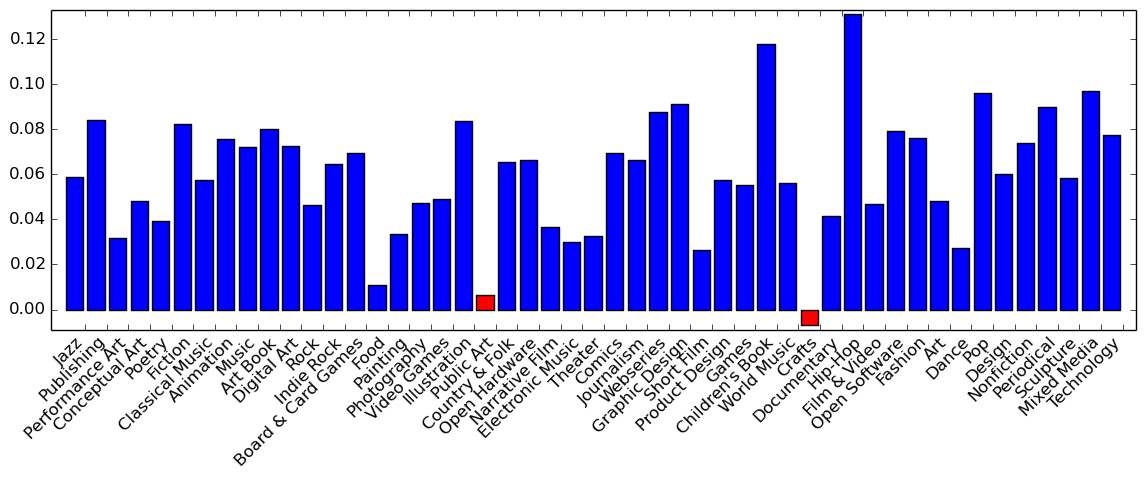
\includegraphics[width=.9\textwidth]{figures/failSuccess.png}                         
\caption{temp}
\label{fig:succfail}
\end{figure*}

\section{Conclusion}

\bibliographystyle{aaai} \bibliography{refs}


\end{document}
